\section{Maths}

There is a lot of material on the web, and on YouTube in particular, that can help explain mathematical things. A favourite on differentiation, integration and related things is Grant Sanderson's \href{https://www.youtube.com/channel/UCYO_jab_esuFRV4b17AJtAw}{``Three Blue One Brown''} YouTube channel, which you will see that we link to at various points below.

\subsection{Derivatives}

Derivatives are just slopes of functions. There are some good videos on the meaning of derivatives and integrals \href{https://www.youtube.com/watch?v=WUvTyaaNkzM&list=PLZHQObOWTQDMsr9K-rj53DwVRMYO3t5Yr}{here}.

Table~\ref{tab:derivatives} shows some derivatives that are useful when manipulating probabilities and likelihood functions.

\begin{table}[ht]
\caption{Some derivative rules. Here $c$ is a constant, $f(\;)$, $g(\;)$ and $h(\;)$ are arbitrary functions, while $x$ and $y$ are variables.
\label{tab:derivatives}}
\begin{minipage}{\linewidth}
\begin{center}
\begin{tabular}{ll}
\hline
Function & Derivative ($f'=\frac{df}{dx}$) \\
\hline
$f(x)=c$ & $f'=0$ \\
$f(x)=x^y$ & $f'=yx^{y-1}$ \\
$f(x)=cg(x)$ & $f'=cg'$ \\
$f(x)=g(x)+h(x)$ & $f'=g'+h'$ \\
$f(x)=\log(x)$ & $f'=\frac{1}{x}$ \\
$f(x)=e^x$ & $f'=e^x$ \\
\hline
$f(x)=\log(x!)$ & $f'\approx\log(x)\footnote{This is an approximation that becomes exact as $x$ approaches $\infty$. (See below if you are unsure what $x!$ means.)}$ \\
\hline
\multicolumn{2}{c}{Chain rule} \\
General: $f(x)=h(g(x))$ & $f'=\frac{dh}{dg}\times\frac{dg}{dx}$ \\
Example 1: $f(x)=\log(g(x))$ & $f'=\frac{1}{g(x)}\times g'$ \\
Example 2: $f(x)=c\log(g(x))$ & $f'=\frac{c}{g(x)}\times g'$ \\
Example 3: $f(x)=e^{cx}$ & $f'= e^{cx}c$ \\
\hline
\end{tabular}
\end{center}
\end{minipage}
\end{table}


\subsection{Integrals}

Integration is just adding things up, but instead of adding discretely (first thing $+$ second thing $+$ third thing $+\cdots$), integration adds continuously. \href{https://www.mathsisfun.com/calculus/integration-introduction.html}{This website} describes the idea in simple terms, and Figure~\ref{fig:integral} illustrates the idea.

\begin{figure}[ht!]
\caption{\small The idea of an integral being the area under a curve, as the limit of a sum of more and more smaller and smaller things. In (a) the interval from -1 to 1.5 has been divided into 20 ``bins'' and the integral is approximated by the sum of the area of each histogram bar. In (b) it has been divided into 50 ``bins'' and we have not plotted the sides of the bins because that makes the plot messy. In (c) it has been divided into 1,000 bins and in this case the bin heights are indistinguishable from the smooth curve.}
\centering
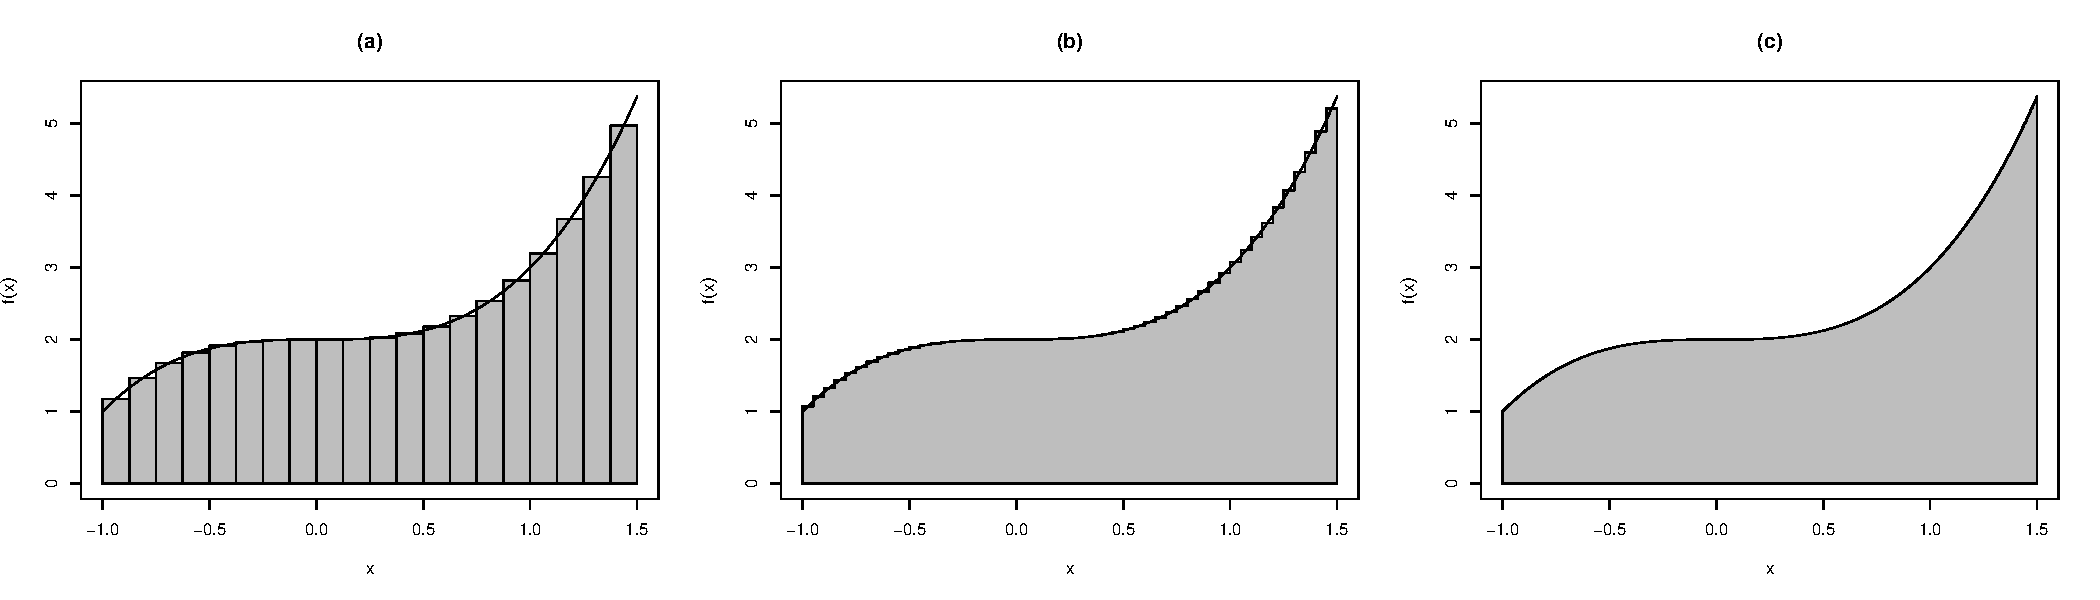
\includegraphics[width=\textwidth]{integralfigure.pdf}
\label{fig:integral}
\end{figure}

Figure~\ref{fig:integral} shows the function $f(x)=x^3+2$ plotted form $x=-1$ to $x=1.5$ as a smooth curve. The area under the curve is approximated by the sum
\be
\sum_{i=1}^K f(m_k)dx \nonumber
\ee
\noindent
where $m_k$ is the midpoint of the $k$th histogram bin, $K$ is the number of bins ($K=20$ in plot (a), $K=50$ in plot (a), $K=1,000$ in plot (c)), and $dx$ is the width of the bins (equal to $[1.5-(-1)]/K$). Notice that $f(m_k)dx$ is the area of the $k$th bin.

In the limit, as $K$ approaches infinity, this sum approaches the true area under the curve between $-1$ and $x=1.5$ (the integral of $x^3$ from -1 to 1.5), i.e., \\
\be
\lim_{K\rightarrow\infty}\sum_{i=1}^K f(m_k)\,dx&= &\int_{-1}^{1.5}f(x)\,dx. \nonumber
\ee

Integrals can be interpreted as \textbf{areas} under curves when integrating in one dimension (as in Figure~\ref{fig:integral}), and as \textbf{volumes} under surfaces when integrating in two dimensions.

\subsubsection{Integral examples}

A typical integral in statistics is the integral under a probability density function (PDF). This area is a probability. For example, the integral from $-\infty$ to $x$ of a the PDF of a standard nomal distribution is the \textbf{probability} that a standard normal random variable is less than or equal to $x$. \href{https://www.youtube.com/watch?v=ZA4JkHKZM50}{Here} is a video that explains how and why areas under PDFs are probabilities.

A different kind of integral that is common in statistical ecology is the integral under an animal density surface. A density surface quantifies the expected number of animals per unit area at any point. Remembering that an integral is just a sum of lots of heights multiplied by tiny widths in one dimenson, or heights multiplied by tiny \textit{areas} in two dimensions, the integral (volume) under the density surface over some region is the expected \textbf{number} of animals in the region (density in each tiny region multiplied by the area of the tiny region, gives the expected number in the tiny region). 

%Often we deal with estimated \textit{expected} density surfaces, and in this case the integral is the \textit{expected number} of animals.

\subsubsection{Computing integrals}

Mathematicians have worked out methods of obtaining formulae for the integrals of many functions. For example, the integral in Figure~\ref{fig:integral} is ($x^4/4+2x$ evaluated at $x=1.5$), minus ($x^4/4+2x$ evaluated at $x=-1$), i.e. $[1.5^4/4+2\times 1.5] - [(-1)^4/4+2\times(-1)] = 6.6.015625$.

The approximations calculated using sums with $K=20$, $K=50$ and $K=1,000$ are 6.013184, 6.015234, and 6.015624, respectively, i.e., they are incorrect by 0.04\%, 0.006\% and 0.00002\%.

It is frequently not possible to obtain formulae for the integrals of functions used in statistical ecology, and we frequently approximate them using sums similar to those shown above (or more sophisticated sums that give better approximations). %When \texttt{R} functions calculate integrals, they invariably used this kind of approximation.


\subsection{Logs}

Here are reminders of equalities involving logs of functions. These are the main ones you will need for routine manipulations of probabilities and likelihood functions.

\be
\log(xy)&=&\log(x)+\log(y) \nonumber \\
\log(x/y)&=&\log(x)-\log(y) \nonumber \\
\log(x^y)&=&y\log(x) \nonumber \\
\ee

Note: We use the ``natural log'' pretty much exclusively. This is log to the base $e$. It is often written as $ln$ rather that $\log$, but we will generally just use $\log$, in part because the \verb|R| has a function \verb|log()| that returns the natural log. 

But what is $e$? It is not crucial that you know what it is, but if you are interested, there are neat explanations \href{https://www.youtube.com/watch?v=AuA2EAgAegE}{here} and \href{https://www.youtube.com/watch?v=m2MIpDrF7Es&t=16s}{here}.

\subsection{Exponentials}

Here are reminders of equalities involving exponentials of functions. These are the main ones you will need for routine manipulations of probabilities and likelihood functions. (Note $e^x$ and $\exp(x)$ are the same thing.)

\be
\exp(x+y)&=&\exp(x)\times\exp(y) \nonumber \\
\exp(x-y)&=&\frac{\exp(x)}{\exp(y)} \nonumber \\
y\exp(x)&=&\exp\{\log(y)\}\times\exp(x)\;=\;\exp\{\log(y) + x\} \nonumber \\
\ee

\subsection{Factorials}

The factorial of an integer is the product of all integers from 1 up to the numebr in question. They are written by writing the number follow by an exclamation mark. So $1!=1$, $2!=1\times 2 = 2$, $3!=1\times 2\times 3 = 6$, $3!=1\times 2\times 3\times 4 = 24$, etc., and $n!=1\times 2\times\ldots\times n$. By convention, $0!=1$.

This $N\choose n$ is read as ``$N$ choose $n$'' and is the number of ways that you can choose $n$ items from $N$ available items (choosing each item at most once). It involves the product and ratio of factorials, thus:

\be
{N\choose n}&=&\frac{N!}{n!(N-n)!}.
\ee